%!TEX TS-program = ../make.zsh

\subsection{Algorithm A: Hole-Ice Propagation as Subsequent Correction of the Propagation Without Hole Ice}
\label{sec:algorithm_a}

% https://github.com/fiedl/hole-ice-study/issues/77

A first approach to adding propagation through hole-ice cylinders to the standard propagation algorithm (section \ref{sec:standardphotonpropagationalgorithm}) implemented in \clsim is to add a subsequent correction to each simulation step without rewriting the existing algorithm.

\sourcepar{The source code of the implementation of this first approach can be found in appendix \ref{sec:algorithm_a_source} as well as in the code repository at \url{https://github.com/fiedl/clsim/tree/sf/hole-ice-2017/resources/kernels/lib/hole_ice}.}

This approach assumes that the scattering length $\lambda\hi\sca$ and the absorption length $\lambda\hi\abs$ within the hole ice can be expressed as multiple of the corresponding scattering length $\lambda\sca$ and absorption length $\lambda\abs$ within the surrounding bulk ice.

$$
  \lambda\sca\hi = f\sca \, \lambda\sca, \ \ \ \lambda\abs\hi = f\abs \, \lambda\abs
$$

The factor $f\sca :\in \reals^+_0$ will be called \textbf{scattering length factor}, $f\abs :\in \reals^+_0$ \textbf{absorption length factor}. These factors can be implemented as properties of the individual hole-ice cylinders, or as common property of all cylinders.

If, for example a cylinder has an absorption length factor of $f\abs = 1$ this means that the absorption length within the hole ice is the same as in the surrounding bulk ice. If the absorption length factor is $f\abs = 0$ this means that the photon will be absorbed instantly when entering the hole-ice cylinder. A scattering factor of $f\sca=0.1$ means that the scattering length within the hole ice is one tenth of the scattering length within the surrounding bulk ice.

\paragraph{Task} The task of this \textbf{hole-ice-correction algorithm} is to modify the quantities that are effected by the hole ice in each simulation step.

Figure \ref{fig:Edahi9sh} illustrates this task: The standard \clsim propagation algorithm calculates the next scattering point $B$ without any knowledge of the hole ice. The hole-ice algorithm takes the properties of the hole ice into account and calculates a correction for the next scattering point. \clsim will use the corrected next scattering point $B'$ rather than the originally calculated point $B$.

\begin{figure}[htbp]
  \smallerimage{photon-trajectory-Edahi9sh}
  \caption{Illustration of the task of the hole-ice correction algorithm. In this two-dimensional scenario, the hole-ice cylinder is represented by a circle. When the photon scatters at point $A$, the standard-\clsim algorithm calculates the next scattering point $B$ without knowledge of the hole ice. The hole-ice correction algorithm calculates what fraction of the trajectory $AB$ runs through the hole ice and determines a correction, resulting in a hole-ice-corrected next scattering point $B'$.}
  \label{fig:Edahi9sh}
\end{figure}

\paragraph{Context} The hole-ice-correction algorithm is inserted into the \clsim propagation algorithm's simulation step right after \clsim has calculated the distance to the next scattering point and the remaining distance to the absorption point without knowledge of the hole ice. After the hole-ice-correction algorithm follows the check whether the photon hits an optical module on the way from $A$ to $B'$.

The hole-ice-correction algorithm takes the following input parameters: Current photon position at point $A$, photon direction after scattering at point $A$, a list of the hole-ice cylinders with their coordinates and radii, the hole-ice scattering length factor $f\sca$ and absorption length factor $f\abs$ as common properties of all hole-ice cylinders, the distance the next scattering point calculated by the standard algorithm, and the remaining distance to the absorption point calculated by the standard algorithm.
As output parameters, the hole-ice correction algorithm returns the hole-ice-corrected distance to the next scattering point and the hole-ice-corrected remaining distance to the absorption point.

\paragraph{Procedure} For each propagation from one scattering point $A$ to the next scattering point $B$, the hole-ice algorithm calculates the intersection points of the photon trajectory $AB$ and the hole-ice cylinders in range.
Based on what portion of the distance $AB$ runs through the hole ice, the algorithm calculates a correction for the distance to the next scattering point and a correction for the remaining distance to the absorption point.

Both calculations, scattering correction and absorption correction, depend on each other: If the photon scatters earlier within the hole ice than determined by the standard algorithm, then the corrected path within the hole ice is shorter than the original one, which means that the remaining distance to the absorption point will be longer as less of the absorption budget is spent, yet.
If, on the other hand, the hole ice absorbs the photon instantly when entering the cylinder, then the corrected final position $B'$ of this simulation step won't be the point determined by the scattering correction but the point where the photon enters the cylinder.

Figure \ref{fig:bahxug7O} shows a flow chart of this algorithm including the loop over the hole-ice cylinders in range, the calculation of the intersection points of photon path and hole-ice cylinder, the correction of the next scattering point and the correction of the remaining distance to absorption.

\begin{figure}[htbp]
  % https://github.com/fiedl/hole-ice-study/issues/77#issuecomment-396559561
  \image{algorithm-hole-ice-2017}
  \caption{Flow chart of the hole-ice-correction algorithm, which calculates subsequent corrections for the quantities that are effected by the hole ice: the distance to the next scattering point and the remaining distance to absorption of the photon. Both corrections depend on each other: If the photon scatters earlier, the absorption correction will be smaller. The algorithm returns the corrected quantities to the standard algorithm, which uses the corrected quantities from that point on.}
  \label{fig:bahxug7O}
\end{figure}

\paragraph{Intersection Calculations} In order to determine the fraction of the path $AB$ of the photon that runs through the hole-ice cylinder, the intersection points of the photon path and the cylinder need to be calculated. This can either be done solving the geometric equations coordinate-wise for the coordinates of the zero, one or two intersection points, or by treating the same scenario as vectorial problem, calculating the coordinate vectors of the intersection points using other vectorial quantities rather than separate coordinates. The latter approach turns out to be more efficient as it utilizes the support of native vector operations of the graphics processing units. Both approaches are presented in appendix \ref{sec:intersections}.

\paragraph{3D-2D Projection}
% https://github.com/fiedl/hole-ice-study/issues/25
% 2017-10-02 2017-10-11 2018-02-07
Intersection points can be calculated in two dimensions by projecting all coordinates from the three-dimensional coordinate system onto the $x$-$y$ plane along the $z$-axis, and then calculating the intersection of a line and a circle rather than the intersections of a line and a cylinder. The fraction of the photon path that runs through the hole ice is the same as in three dimensions due to the intercept theorem, because both, the distance to the intersection point, $\len{AX}_\text{2D}:=\xi \len{AX}_\text{3D}$, and the distance to the next scattering point, $\len{AB}_\text{2D}:=\xi \len{AB}_\text{3D}$, use the same projection factor $\xi \in \reals^+$, which itself depends on the photon direction.

$$
  \frac{\len{AX}_\text{2D}}{\len{AB}_\text{2D}} = \frac{\len{AX}_\text{3D}}{\len{AB}_\text{3D}}
$$

The relative distance corrections, $\sfrac{\Delta x}{\len{AB}}$, are the same in two and three dimensions due to the same reason. But the absolute distance correction $\Delta x : \len{AB'} = \len{AB} + \Delta x$ needs to be expressed in three dimensions when adding the correction to the distances used in the standard algorithm as they are defined for a three-dimensional coordinate system.
Keeping this conversion requirement in mind, the geometric cases of the photon path $AB$ running through a hole-ice cylinder can be examined in two dimensions.

\paragraph{Geometric Cases}
% https://github.com/fiedl/hole-ice-study/issues/77#issuecomment-396581950
% https://github.com/fiedl/hole-ice-study/issues/2 -- corrections for $f > 1$
% https://github.com/fiedl/hole-ice-study/issues/20 -- missing geometric test cases
%
When the hole-ice algorithm calculates the distance correction $\Delta x: \len{AB'} = \len{AB} + \Delta x$, there are several geometric cases to consider, depending on the number $N$ of intersections of the photon path $AB$ with the hole-ice cylinder and whether the path starts within the cylinder or outside the cylinder.

\begin{figure}[htbp]
  \smallerimage{intersection-iefai4iV}
  \caption{Intersection of the line along the photon path $AB$ with the hole-ice cylinder in two dimensions, where the cylinder is represented by a circle of radius $r$ around the center $M$. The first intersection point is $Y$, the second intersection point $X$. The second intersection point $X$ is beyond the path's end point $B$. Thus, the number $N$ of intersections is considered to be $N=1$ in this case.}
  \label{fig:iefai4iV}
\end{figure}

The distance correction depends on the fraction $w :\in \reals^+_0$ of the path length $\len{AB}$ that runs within the hole-ice cylinder.

\begin{description}
  \item[Case 1] If the photon starts outside the cylinder and the path has no intersection with the cylinder ($N = 0$), then the path does not run through the cylinder, $w = 0$, and the distance correction $\Delta x$ needs to be zero: $\Delta x = 0$.
  \item[Case 2] If the photon starts inside the cylinder and the path has no intersection with the cylinder ($N = 0$), then the whole path is within the cylinder, $w = 1$. A photon that would travel a distance of $\lambda$ within the bulk ice, travels a distance of $\lambda\hi$ within the hole ice, $\lambda\hi = f\,\lambda$. The distance correction $\Delta x$ for this photon would be $\Delta x = \lambda\hi - \lambda = (f - 1)\lambda$, or more generally, $\Delta x = (f - 1) \len{AB}$.
  \item[Case 3] If the photon starts outside the cylinder, but intersects the cylinder once ($N = 1$), then the first part of the trajectory, $AY$, stays the same, and only the path from the first intersection point $Y$ to the destination point $B$ runs within the hole ice, $w = \len{YB} / \len{AB}$. As only this fraction needs to be corrected, the distance correction is $\Delta x = (f - 1)\len{YB}$.
  \item[Case 4] If the photon intersects the cylinder once ($N = 1$), but starts within the cylinder, only the first part, $AC$, of the path needs to be corrected.

  $C$ is the \textbf{termination point} of the trajectory inside the cylinder. In cases where the photon reaches the far end of the cylinder, $C$ is just the second intersection point, $C = X$. If the trajectory within the cylinder is terminated, however, by the other interaction respectively, for example if the photon is scattered away before reaching the far end when calculating the absorption correction, $C$ is the point where the trajectory is terminated by the other interaction.
    % termination point formalsim: 2017-10-10 2017-10-13 2018-02-02

  In contrast to Case 3 where the outside distance $\len{AY}$ has been fixed, in this case the outside trajectory part $\len{CB}$ comes after the hole-ice part $\len{YC}$ and will be the shorter the stronger the hole-ice correction is. Therefore, one needs to use the scaled distance $\len{AC} / f$ to determine how much of the path will remain outside the cylinder, resulting in a distance correction of $\Delta x = (1 - \frac{1}{f})\len{AC}$.
  \item[Case 5] If the photon starts outside the cylinder and has two intersections ($N = 2$) with the cylinder, this is a combination of Case 3 and Case 4, resulting in a distance correction of $\Delta x = (1 - \frac{1}{f})\len{YC}$.
\end{description}

A flow chart of the distance-correction algorithm is shown in figure \ref{fig:Eeshi4Oh}.

\begin{figure}[htbp]
  % https://github.com/fiedl/hole-ice-study/issues/77#issuecomment-396581950
  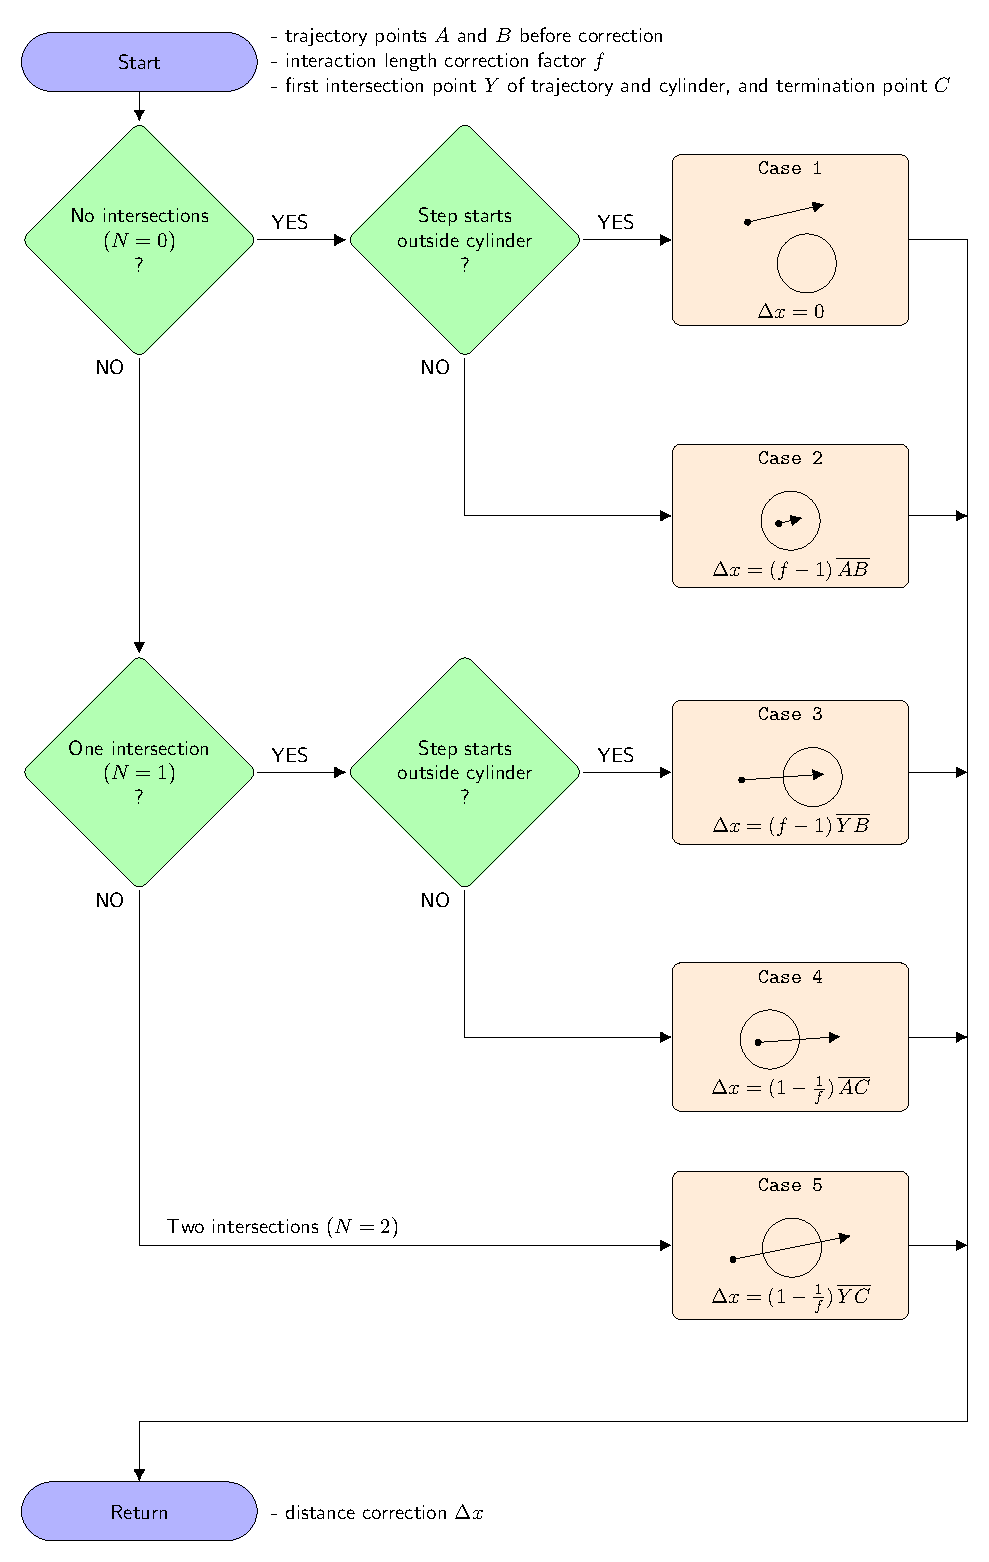
\includegraphics[height=\textheight]{img/algorithm-hole-ice-correction-2017-case-ordered}
  \caption{Flow chart for calculating the hole-ice correction for the geometric distance to the next interaction point.}
  \label{fig:Eeshi4Oh}
\end{figure}

\paragraph{Pros and Cons}
As this first hole-ice algorithm only adds subsequent corrections for the standard-\clsim algorithm, it leaves the standard-\clsim code, which is already well tested, almost untouched.
The additions of the hole-ice algorithm interface with the \clsim algorithm only through a small surface area, corresponding to a small number of variables passed from one algorithm to the other. This allows to test the hole-ice algorithm with so-called \textit{unit tests} (section \ref{sec:unit_tests}) where specific examples with fixed input variables are provided and tested whether the algorithm produces the expected results for the example.

The hole-ice correction algorithm, however, has important limitations.
First, the current understanding of the hole ice suggests that the interaction properties of the hole ice are independent of the properties of the surrounding bulk ice (see section \ref{sec:hole_ice}). But with this hole-ice correction algorithm, it is only possible to define the interaction lengths of the hole ice relative to the interaction properties of the surrounding bulk ice.
While one could workaround this problem locally by adjusting the correction factors $f$ in relation to the local properties of the bulk ice, large jumps over several layers of ice with different properties would cause inevitable errors.

Secondly, the algorithm does work only correct in scenarios where the photon crosses only one cylinder between two scattering points. In scenarios where the photon crosses several cylinders, for example when nested cylinders are used to model radially changing properties of the hole ice, or when instantly-absorbing cylinders are used to model cables within a hole-ice cylinder, this algorithm is not able to calculate the corrections properly because it would interpret the interaction factors $f$ not only relative to the surrounding bulk ice but also relative to the cylinders the photon has already crossed in this simulation step.

A different approach to adding propagation through hole-ice cylinders to the standard-propagation algorithm is to treat hole-ice cylinders the same way as other media such as ice layers rather than accounting for the hole-ice effects using ex-post corrections. This second approach gets rid of the above shortcomings, but at the cost that the standard-\clsim algorithm that handles the propagation through different media needs to be re-written. This second approach is described in the following section.